
\documentclass{beamer}
\usecolortheme{dove}
\setbeamertemplate{navigation symbols}{}
\usepackage{amsmath,amssymb,amsfonts,amsthm, multicol, subfigure, color}
\usepackage{bm}
\usepackage{graphicx}
\usepackage{tabularx}
\usepackage{booktabs}
\usepackage{hyperref}
\usepackage{pdfpages}
\usepackage{xcolor}
\definecolor{seagreen}{RGB}{46, 139, 87}
\definecolor{mustard}{RGB}{234, 170, 0}
\def\independenT#1#2{\mathrel{\rlap{$#1#2$}\mkern2mu{#1#2}}}
\newcommand\indep{\protect\mathpalette{\protect\independenT}{\perp}}
\def\log{\text{log}}
\newcommand\logit{\text{logit}}
\newcommand\iid{\stackrel{\text{iid}}{\sim}}
\newcommand\E{\text{E}}
\newcommand\V{\text{V}}
\renewcommand\P{\text{P}}
\newcommand{\Cov}{\text{Cov}}
\newcommand{\Cor}{\text{Cor}}
\newcommand\doop{\texttt{do}}
\usepackage{stackrel}
\usepackage{tikz}
\usetikzlibrary{arrows,shapes.arrows,positioning,shapes,patterns,calc}
\newcommand\slideref[1]{\vskip .1cm \tiny \textcolor{gray}{{#1}}}
\newcommand\red[1]{\color{red}#1}
\newcommand\blue[1]{\color{blue}#1}
\newcommand\gray[1]{\color{gray}#1}
\newcommand\seagreen[1]{\color{seagreen}#1}
\newcommand\purple[1]{\color{purple}#1}
\newcommand\orange[1]{\color{orange}#1}
\newcommand\black[1]{\color{black}#1}
\newcommand\white[1]{\color{white}#1}
\newcommand\teal[1]{\color{teal}#1}
\newcommand\magenta[1]{\color{magenta}#1}
\newcommand\Fuchsia[1]{\color{Fuchsia}#1}
\newcommand\BlueGreen[1]{\color{BlueGreen}#1}
\newcommand\bblue[1]{\textcolor{blue}{\textbf{#1}}}
\newcommand\bred[1]{\textcolor{red}{\textbf{#1}}}
\newcommand\bgray[1]{\textcolor{gray}{\textbf{#1}}}
\newcommand\bgreen[1]{\textcolor{seagreen}{\textbf{#1}}}
\newcommand\bref[2]{\href{#1}{\color{blue}{#2}}}
\colorlet{lightgray}{gray!40}
\pgfdeclarelayer{bg}    % declare background layer for tikz
\pgfsetlayers{bg,main} % order layers for tikz
\newcommand\mycite[1]{\begin{scriptsize}\textcolor{darkgray}{(#1)}\end{scriptsize}}
\newcommand{\tcframe}{\frame{
%\small{
\only<1|handout:0>{\tableofcontents}
\only<2|handout:1>{\tableofcontents[currentsubsection]}}
%}
}

\newcommand{\goalsframe}{\begin{frame}{Learning goals for today}
By the end of class, you will be able to
\begin{itemize}
    \item study education as an intervention\\that might change inequality
\end{itemize} \vskip .2in
\end{frame}}

\usepackage[round]{natbib}
\bibliographystyle{humannat-mod}
\setbeamertemplate{enumerate items}[default]
\usepackage{mathtools}

\title{Studying Social Inequality with Data Science}
\author{Ian Lundberg}
\date{\today}

\begin{document}

\begin{frame}
\begin{tikzpicture}[x = \textwidth, y = \textheight]
\node at (0,0) {};
\node at (1,1) {};
\node[anchor = north west, align = left, font = \huge] at (0,.9) {Studying\\Social Inequality\\with Data Science};
\node[anchor = north east, align = right] (number) at (1,.9) {INFO 3370 / 5371\\Spring 2023};
\node[anchor = north, font = \Large, align = left] at (.5,.5) {\bblue{Interventions to Promote Equality:}\\\bblue{Educational Expansion}};
\end{tikzpicture}
\end{frame}

\goalsframe

\begin{frame}{A motivating research study}

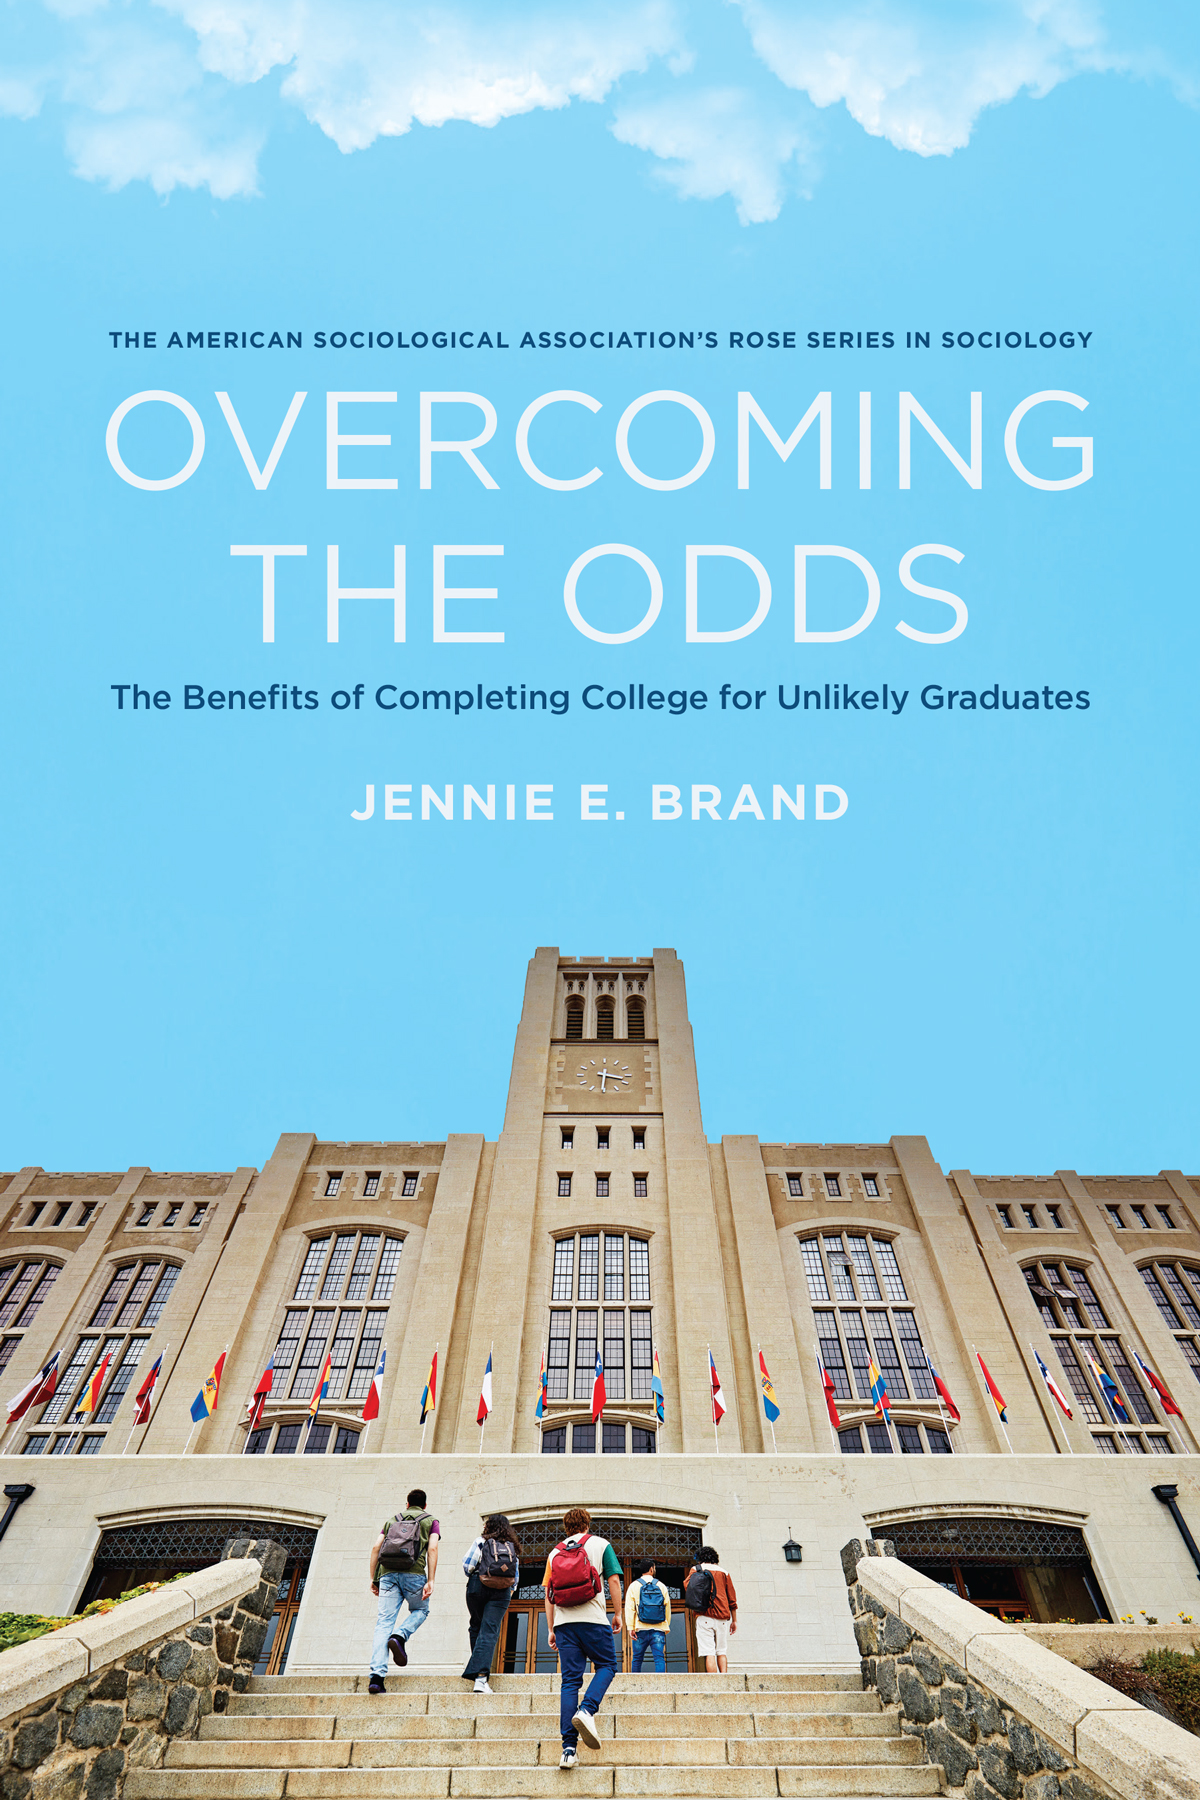
\includegraphics[height = .8\textheight]{figures/brand_cover}

\end{frame}

\begin{frame}

Americans' education in 1900\hfill \mycite{Brand 2023 p.~6}
\begin{itemize}
\item 6\% graduated from high school
\item 3\% graduated from college
\end{itemize}

\end{frame}

\begin{frame}

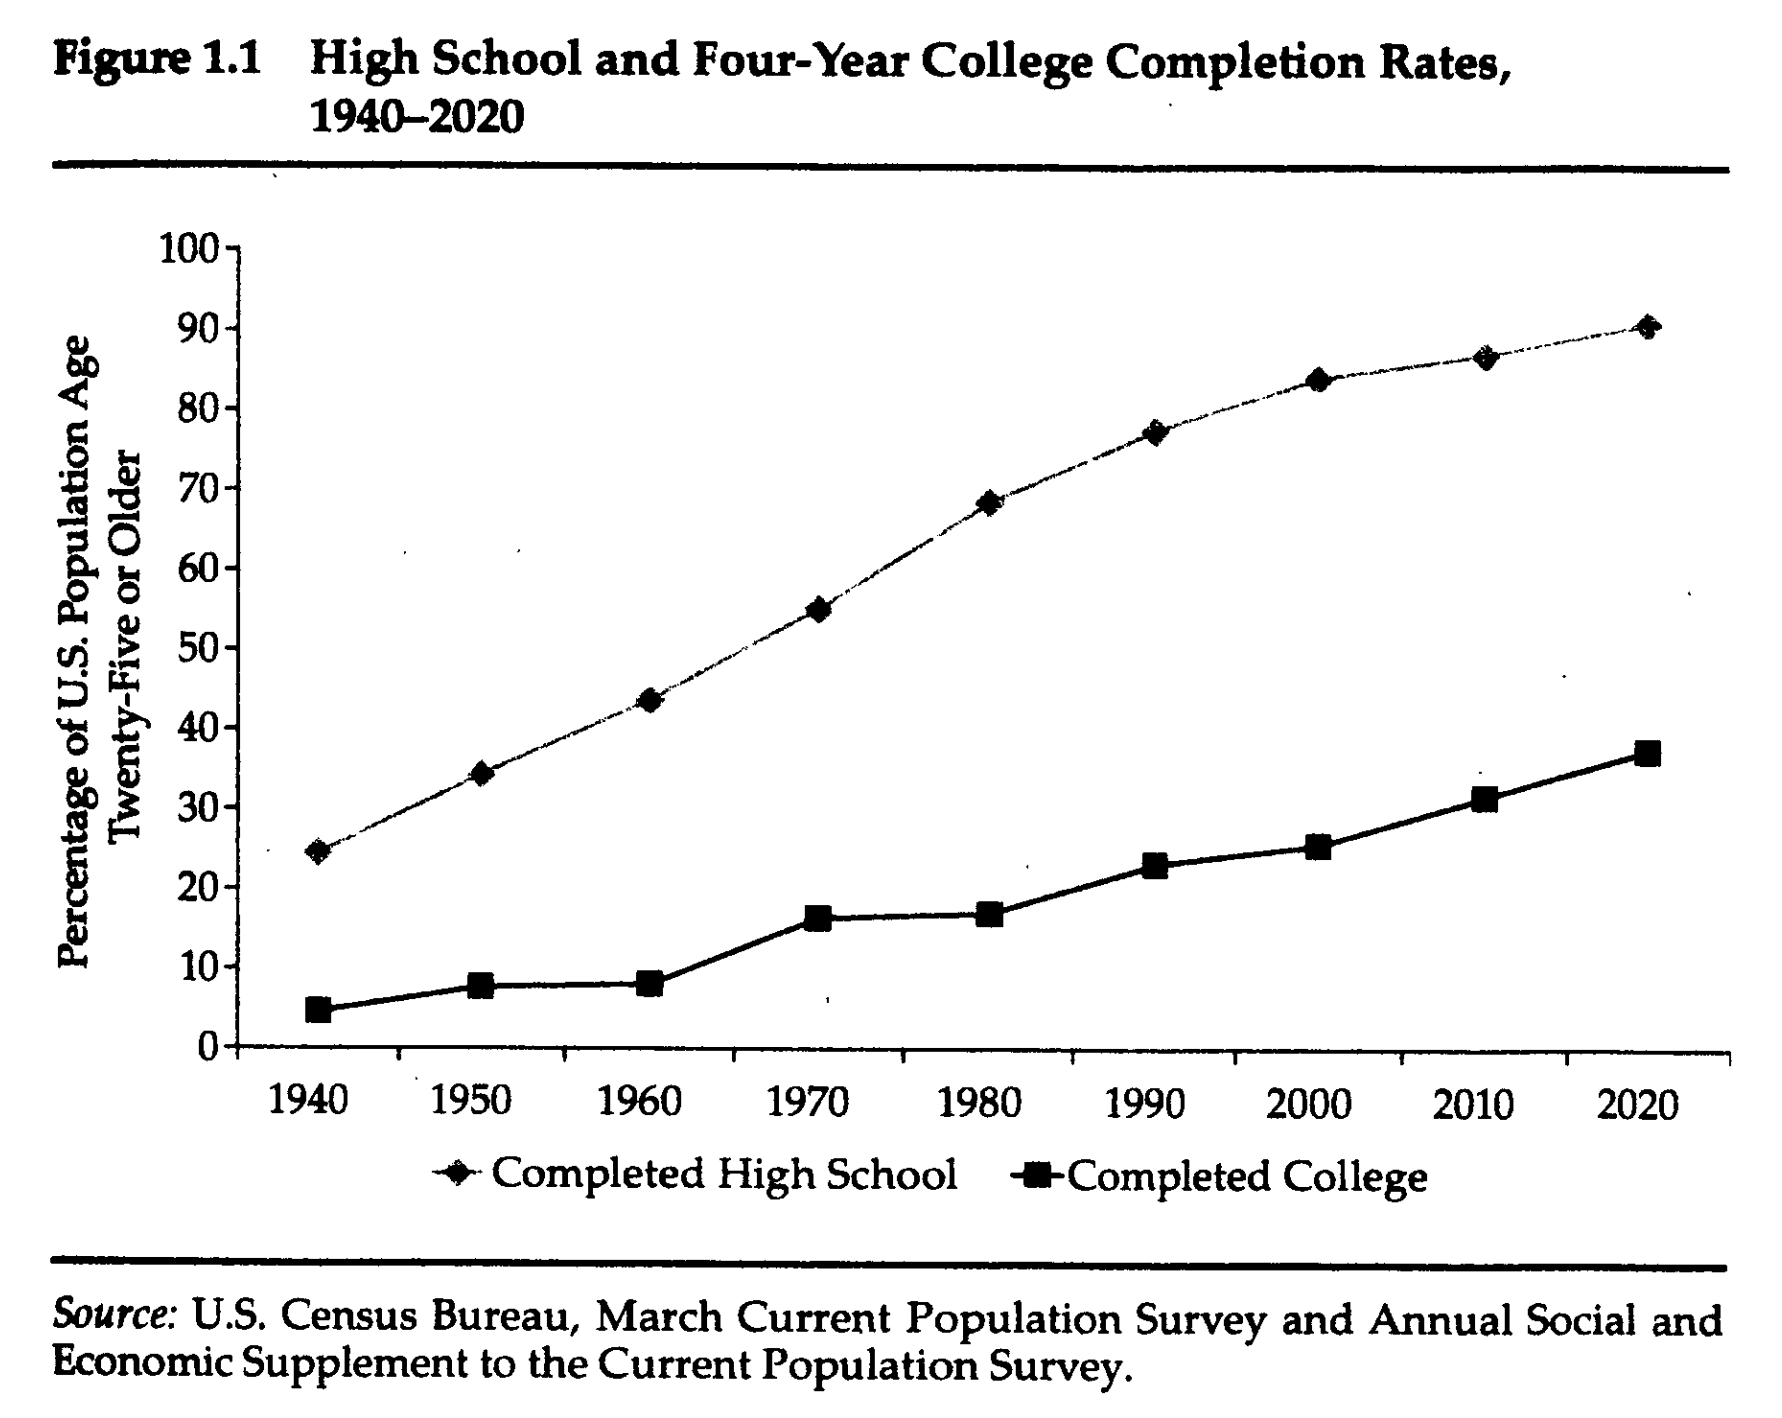
\includegraphics[width = .9\textwidth]{figures/brand_fig1}\\\hfill\mycite{Brand 2023}

\end{frame}

\begin{frame}{Why did education expand?} \pause
\begin{itemize}
\item Public investment in college
\begin{itemize}
\item Morrill Act (1862) sold land to establish colleges
\item G.I. Bill (1944) funded veterans' college
\end{itemize} \pause
\item Rising labor market demand for skills
\end{itemize}
\end{frame}

\begin{frame}{Investment changes: From institutions to students} \pause
\begin{itemize}
\item Higher Education Act (1965) created Pell Grants
\item Federal student loans
\end{itemize} \vskip .2in \pause
Consequences \pause
\begin{enumerate}
\item Growing perception that individuals (not states)\\ought to bear the cost of college \pause
\item Privatization of college \pause
\end{enumerate} \vskip .2in
Open question: Should we invest more? How would we decide?

\end{frame}

\begin{frame}

We would like to know whether \textbf{college pays off}:\\
does it have positive effects on desired outcomes?

\end{frame}

\begin{frame}{Does college pay off? A hypothetical experiment} \pause

\begin{itemize}
\item randomly sample high school students \pause
\item randomize them to either
\begin{itemize}
\item stop education after a high school degree, or
\item complete a 4-year degree \pause
\end{itemize}
\item compare adult wages
\end{itemize}

\end{frame}

\begin{frame}{Does college pay off? An observational study}{Brand 2023 p.~44, 69, 116--117}

\scalebox{.7}{
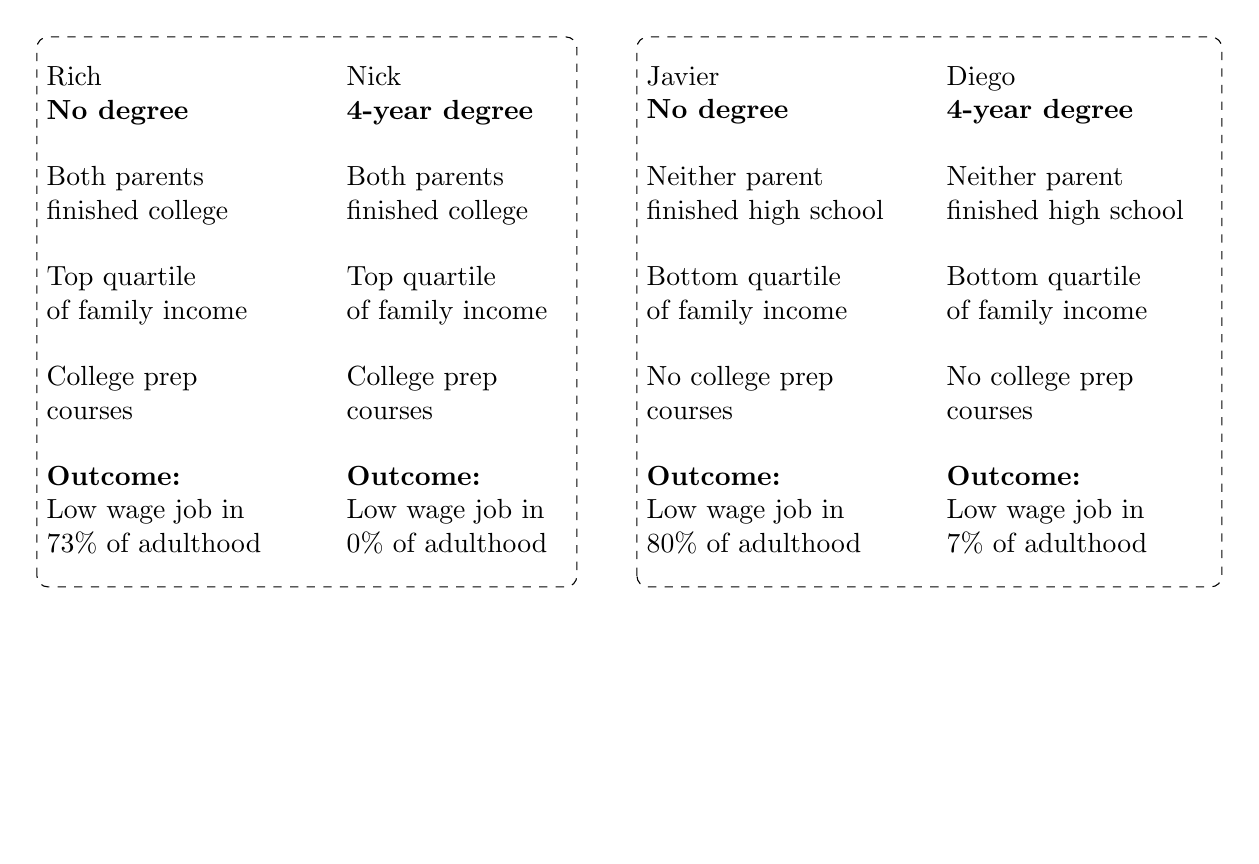
\begin{tikzpicture}[x = 1.5in, y = .5in]
\node at (1,.2) {};
\node at (4.95,-7.7) {};
\node<11->[anchor = north west, align = left] at (1,0) {Rich\\\textbf{No degree}};
\onslide<12->{
\node[anchor = north west, align = left] at (1,-1) {Both parents\\finished college};
\node[anchor = north west, align = left] at (1,-2) {Top quartile\\of family income};
\node[anchor = north west, align = left] at (1,-3) {College prep\\courses};
}
\node<13->[anchor = north west, align = left] at (1,-4) {\textbf{Outcome:}\\Low wage job in\\73\% of adulthood};
\node<2->[anchor = north west, align = left] at (2,0) {Nick\\\textbf{4-year degree}};
\node<3->[anchor = north west, align = left] at (2,-1) {Both parents\\finished college};
\node<4->[anchor = north west, align = left] at (2,-2) {Top quartile\\of family income};
\node<5->[anchor = north west, align = left] at (2,-3) {College prep\\courses};
\node<6->[anchor = north west, align = left] at (2,-4) {\textbf{Outcome:}\\Low wage job in\\0\% of adulthood};
\node<2->[anchor = north west, align = left] at (3,0) {Javier\\\textbf{No degree}};
\node<7->[anchor = north west, align = left] at (3,-1) {Neither parent\\finished high school};
\node<8->[anchor = north west, align = left] at (3,-2) {Bottom quartile\\of family income};
\node<9->[anchor = north west, align = left] at (3,-3) {No college prep\\courses};
\node<10->[anchor = north west, align = left] at (3,-4) {\textbf{Outcome:}\\Low wage job in\\80\% of adulthood};
\onslide<15->{
\node[anchor = north west, align = left] at (4,0) {Diego\\\textbf{4-year degree}};
\node[anchor = north west, align = left] at (4,-1) {Neither parent\\finished high school};
\node[anchor = north west, align = left] at (4,-2) {Bottom quartile\\of family income};
\node[anchor = north west, align = left] at (4,-3) {No college prep\\courses};
\node[anchor = north west, align = left] at (4,-4) {\textbf{Outcome:}\\Low wage job in\\7\% of adulthood};
}
\draw<14->[dashed, rounded corners] (1,-5.3) rectangle (2.8, .2);
\draw<16->[dashed, rounded corners] (3,-5.3) rectangle (4.95, .2);
%\node<17->[anchor = north west, font = \LARGE] (why) at (1,-5.8) {Why are these comparisons more compelling?};
%\node<18->[anchor = north west, align = left, font = \LARGE] at (why.south west) {They approximate \textbf{counterfactuals}:\\Same person, different treatment};
\end{tikzpicture}}

\end{frame}

\begin{frame}{Mathematical notation for two types of claims}


\begin{tikzpicture}[x = \textwidth, y = .8\textheight]
\node at (0,0) {};
\node at (1,1) {};
\node<2->[anchor = north west, align = left] at (.05,1) {People with\\college degrees\\earn more};
\node<2->[anchor = north west, align = left] at (.55,1) {A college degree\\causes\\higher earnings};
\node<3-6>[anchor = north west, align = left] at (0.05,.7) {Two sets of people\\Two treatments};
\only<4->{
\draw[rounded corners, fill = blue, fill opacity = .3] (.05,.3) rectangle (.25,.5) {};
\draw[rounded corners, fill = seagreen, fill opacity = .3] (.25,.1) rectangle (.45,.3) {};
\node[anchor = north, align = center, font = \footnotesize, blue] at (.15, .1) {Outcome\\with college};
\node[anchor = north, align = center, font = \footnotesize, seagreen] at (.35, .1) {Outcome\\without};
\node[anchor = south, rotate = 90, align = center] at (.05, .3) {People};
}
\node<5-7>[anchor = north west, align = left] at (.55,.7) {Same people\\Two treatments};
\only<6->{
\draw[rounded corners, fill = blue, fill opacity = .3] (.55,.1) rectangle (.75,.5) {};
\draw[rounded corners, fill = seagreen, fill opacity = .3] (.75,.1) rectangle (.95,.5) {};
\node[anchor = north, align = center, font = \footnotesize, blue] at (.65, .1) {Outcome\\with college};
\node[anchor = north, align = center, font = \footnotesize, seagreen] at (.85, .1) {Outcome\\without};
\node[anchor = south, rotate = 90, align = center] at (.55, .3) {People};
}
\node<7-> at (.15, .4) {$Y_i$};
\node<7-> at (.35, .2) {$Y_i$};
\node<8-> at (.65, .3) {$Y_i^\text{College}$};
\node<8->[font = \small] at (.85, .3) {$Y_i^\text{Non-college}$};
\only<7->{
\node[anchor = north, align = center] (factual) at (.25,.7) {factual\\outcomes};
\draw[->, thick] (.2,.55) -- (.15,.45);
\draw[->, thick] (.3,.55) -- (.35,.25);
}
\only<8->{
\node[anchor = north, align = center] (potential) at (.75,.7) {potential\\outcomes};
\draw[->, thick] (.7,.55) -- (.65,.35);
\draw[->, thick] (.8,.55) -- (.85,.35);
}
\node<8->[anchor = north east, align = right, font = \footnotesize, gray] at (1,.7) {\href{https://catalog.library.cornell.edu/catalog/12108069}{Imbens \&}\\\href{https://catalog.library.cornell.edu/catalog/12108069}{Rubin}\\\href{https://catalog.library.cornell.edu/catalog/12108069}{2015}};
\end{tikzpicture}

\end{frame}

\begin{frame}{\only<1-3>{The fundamental problem of causal inference}\only<4->{Solving the problem: Assumptions \hfill (Exchangeability)}}
\begin{tikzpicture}[x = \textwidth, y = .8\textheight]
\node at (0,0) {};
\node at (1,1) {};
\node<1-3>[anchor = south east, gray, font = \bf] at (1,0) {\href{https://www.tandfonline.com/doi/abs/10.1080/01621459.1986.10478354}{Holland 1986}};
% Individual outcomes
\node[anchor = north west, font = \bf] at (.05,1) {The data};
\foreach \i in {.5,.7,.8} {
	\draw[fill = blue, opacity = .3, color = blue] (.05,\i) rectangle (.25,\i + .1) {};
}
\foreach \i in {.3,.4,.6} {
	\draw[fill = seagreen, opacity = .3, color = seagreen] (.25,\i) rectangle (.45,\i + .1) {};
}
\node[font = \footnotesize] at (.15,.85) {$Y_\text{Nick}^\text{College}$};
\node[font = \footnotesize] at (.15,.75) {$Y_\text{William}^\text{College}$};
\node[font = \footnotesize] at (.35,.65) {$Y_\text{Rich}^\text{Non-college}$};
\node[font = \footnotesize] at (.15,.55) {$Y_\text{Diego}^\text{College}$};
\node[font = \footnotesize] at (.35,.45) {$Y_\text{Javier}^\text{Non-college}$};
\node[font = \footnotesize] at (.35,.35) {$Y_\text{Jes\'us}^\text{Non-college}$};
\node[anchor = north, align = center, font = \footnotesize, blue] at (.15, .3) {Outcome\\under\\treatment};
\node[anchor = north, align = center, font = \footnotesize, seagreen] at (.35, .3) {Outcome\\under\\control};
\node[anchor = south, rotate = 90, align = center] at (.05, .6) {Each Row is a Person};
% The claim
\onslide<2->{
\node[anchor = north west, font = \bf] at (.55,1) {The claim};
\foreach \i in {.3,.4,.5,.6,.7,.8} {
	\draw[fill = blue, opacity = .3, color = blue] (.55,\i) rectangle (.75,\i + .1) {};
	\draw[fill = seagreen, opacity = .3, color = seagreen] (.75,\i) rectangle (.95,\i + .1) {};
	\draw[<->, thick] (.73,\i + .05) -- (.77,\i + .05);
}
\node[font = \footnotesize] at (.65,.85) {$Y_\text{Nick}^\text{College}$};
\node[font = \footnotesize] at (.85,.85) {$Y_\text{Nick}^\text{Non-college}$};
\node[font = \footnotesize] at (.65,.75) {$Y_\text{William}^\text{College}$};
\node[font = \footnotesize] at (.85,.75) {$Y_\text{William}^\text{Non-college}$};
\node[font = \footnotesize] at (.65,.65) {$Y_\text{Rich}^\text{College}$};
\node[font = \footnotesize] at (.85,.65) {$Y_\text{Rich}^\text{Non-college}$};
\node[font = \footnotesize] at (.65,.55) {$Y_\text{Diego}^\text{College}$};
\node[font = \footnotesize] at (.85,.55) {$Y_\text{Diego}^\text{Non-college}$};
\node[font = \footnotesize] at (.65,.45) {$Y_\text{Javier}^\text{College}$};
\node[font = \footnotesize] at (.85,.45) {$Y_\text{Javier}^\text{Non-college}$};
\node[font = \footnotesize] at (.65,.35) {$Y_\text{Jes\'us}^\text{College}$};
\node[font = \footnotesize] at (.85,.35) {$Y_\text{Jes\'us}^\text{Non-college}$};
\node[anchor = north, align = center, font = \footnotesize, blue] at (.65, .3) {Outcome\\under\\treatment};
\node[anchor = north, align = center, font = \footnotesize, seagreen] at (.85, .3) {Outcome\\under\\control};
}
\node<3>[anchor = north west] at (0,.06) {Counterfactuals are \textbf{not observed}};
\onslide<3->{
\node[font = \footnotesize] at (.35,.85) {?};
\node[font = \footnotesize] at (.35,.75) {?};
\node[font = \footnotesize] at (.15,.65) {?};
\node[font = \footnotesize] at (.35,.55) {?};
\node[font = \footnotesize] at (.15,.45) {?};
\node[font = \footnotesize] at (.15,.35) {?};
}
\draw<5-> (.05,.6) rectangle (.45,.9);
\draw<5-> (.05,.3) rectangle (.45,.6);
\draw<6->[->, thick] (.3, .68) to[out = 90, in = 215] (.33,.73);
\draw<6->[->, thick] (.3, .68) to[out = 90, in = 215] (.33,.83);
\draw<7->[->, thick] (.1, .83) to[out = 215, in = 150] (.13,.65);
\draw<7->[->, thick] (.1, .73) to[out = 215, in = 150] (.13,.65);
\draw<8->[->, thick] (.116, .53) to[out = 270, in = 150] (.14,.47);
\draw<8->[->, thick] (.116, .53) to[out = 270, in = 150] (.14,.37);
\draw<9->[->, thick] (.3, .47) to[out = 115, in = 210] (.33,.53);
\draw<9->[->, thick] (.28, .37) to[out = 145, in = 210] (.33,.53);
\end{tikzpicture}
\end{frame}

\begin{frame}{Quick review} \pause

\begin{enumerate}
\item causal effects involve missing data
\begin{itemize}
\item Nick finished college college
\item outcome without college is unobserved
\end{itemize} \pause
\item randomization solves the missing data problem by design
\begin{itemize}
\item treated and control groups are exchangeable
\end{itemize} \pause
\item observational studies solve the missing data problem by assumptions
\begin{itemize}
\item find population subgroups who look similar before treatment
\item assume it is like an experiment within the subgroups
\end{itemize}
\end{enumerate} %\vskip .2in
%\textbf{Next:} In what ways should Nick's matches look like him?

\end{frame}

\begin{frame}

Concrete example: Research questions and empirical evidence

\end{frame}

\begin{frame}{Studying the effect of college}{Source: Brand 2023}

Data
\begin{itemize}
\item probability samples of children 14--22 in 1979 and 12--17 in 1997
\item measurement of pre-college characteristics
\item measurement of four-year completion
\item many outcome variables in adulthood
\begin{itemize}
\item earnings, unemployment, low-wage work, etc
\item household income, family poverty, marriage, etc
\item social assistance receipt
\item volunteering, voting, etc
\end{itemize}
\end{itemize}

\end{frame}

\begin{frame}{Who benefits the most from college?}{Source: Brand 2023} \pause

A summary of advantage: The propensity score
$$\P(\text{College}\mid \text{Measured Pre-College Variables})$$ \vskip .3in
(technically: the measured variables must be sufficient for conditional exchangeability to hold)

\end{frame}

\begin{frame}{Who benefits the most from college?}{Source: Brand 2023}

Who benefits most from college:

\begin{itemize}
\item those likely to finish college \hfill (advantaged)
\item those unlikely to finish college \hfill (disadvantaged)
\end{itemize}

\end{frame}

\begin{frame}{Who benefits the most from college?}{Source: Brand 2023}

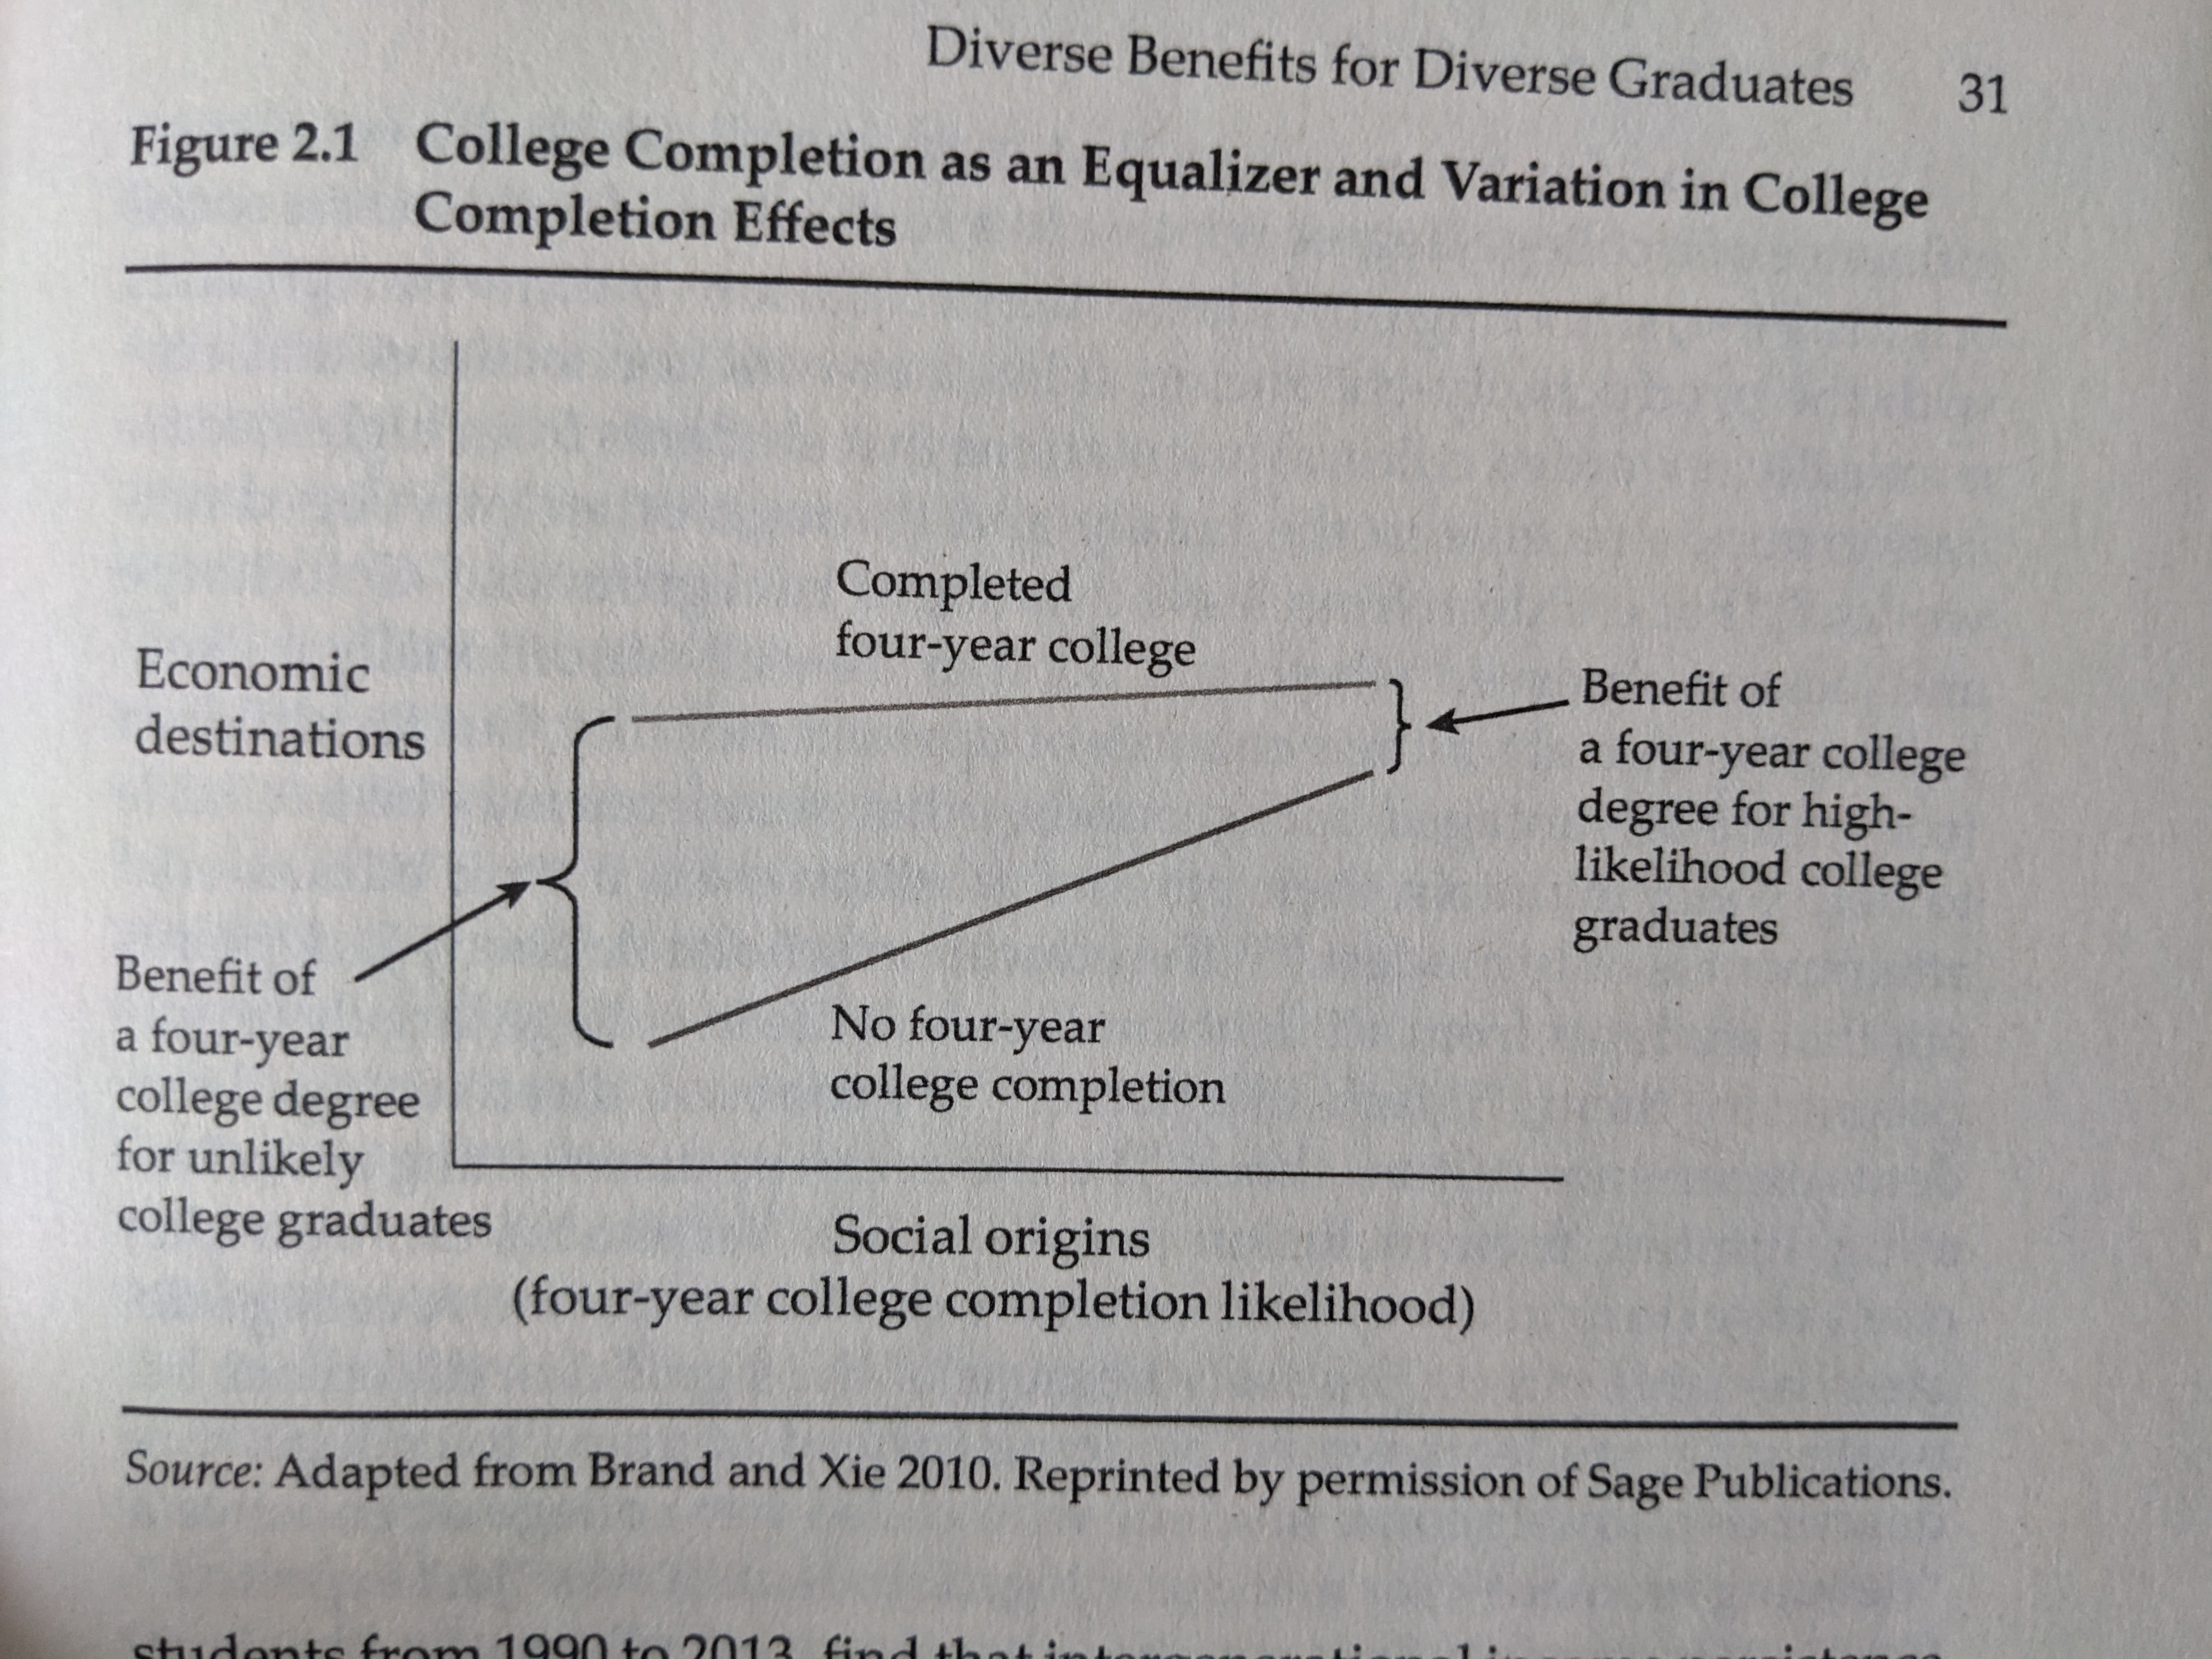
\includegraphics[width = .8\textwidth]{figures/brand_p31}

\end{frame}

\begin{frame}{Causal identification}{Brand 2023 p.~74 for measured variable list}

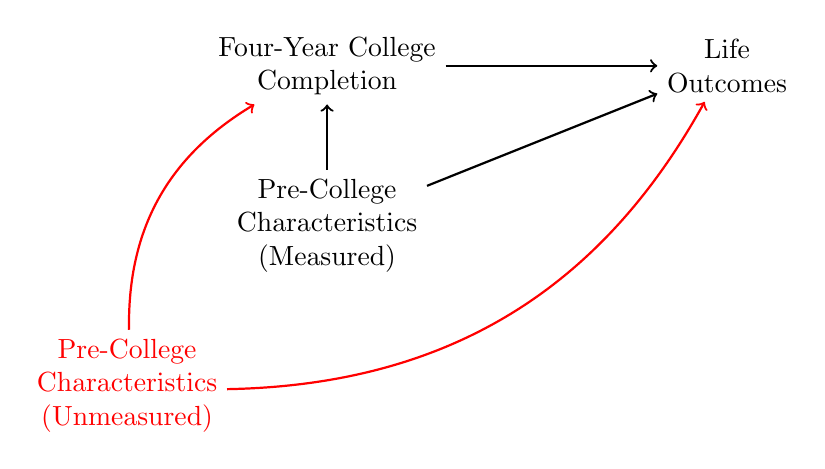
\begin{tikzpicture}[x = 1in, y = .8in]
\node[align = center] (x) at (0,-1) {Pre-College\\Characteristics\\(Measured)};
\node[align = center] (y) at (2,0) {Life\\Outcomes};
\node[align = center] (a) at (0,0) {Four-Year College\\Completion};
\draw[->, thick] (x) -- (a);
\draw[->, thick] (x) -- (y);
\draw[->, thick] (a) -- (y);
\node[align = center, red] (u) at (-1,-2) {Pre-College\\Characteristics\\(Unmeasured)};
\draw[->, thick, red] (u) to[bend left] (a);
\draw[->, thick, red] (u) to[bend right] (y);
\end{tikzpicture}

\end{frame}

\begin{frame}{Estimation}{Brand 2023 p.~84} \pause

\begin{itemize}
\item logistic regression to predict college completion \pause
\item restrict to region of common support
\begin{itemize}
\item $\geq$ 0.3\% chance of college completion
\item $\leq$ 92.3\% chance of college completion
\end{itemize}  \pause
\item match each college graduate to a non-graduate\\with similar probability of college completion  \pause
\item report estimates for three groups
\begin{itemize}
\item low propensity of college completion \hfill 0.3--20\%
\item middle propensity of college completion \hfill 20--50\%
\item high propensity of college completion \hfill 50--92.3\%
\end{itemize}
\end{itemize}

\end{frame}


\begin{frame}{An intervention to \textbf{reduce inequality}}

\includegraphics<1>[width = .8\textwidth]{figures/brand_p31}
\includegraphics<2>[width = .8\textwidth]{figures/brand_wage}
\includegraphics<3>[width = .8\textwidth]{figures/brand_unemployment}
\includegraphics<4>[width = .8\textwidth]{figures/brand_household}

\end{frame}


\begin{frame}
Next week: On what should we match?
\end{frame}

\begin{frame}
\begin{tikzpicture}[x = \textwidth,y = \textheight]
\node at (0,0) {};
\node at (1,1) {};
\foreach \i in {1,...,36} {
	\node<\i>[anchor = north west] at (0,1) {\includegraphics[page = \i, width = .9\textwidth]{causal_assumptions_existing_slides}};
}
\end{tikzpicture}
\end{frame}

\begin{frame}{Recap: Causal effect of college on earnings}

\begin{enumerate}
\item Fundamental problem: Counterfactuals not observed
\item Assume a DAG: enumerate causal processes creating association between education and earnings
\begin{center}
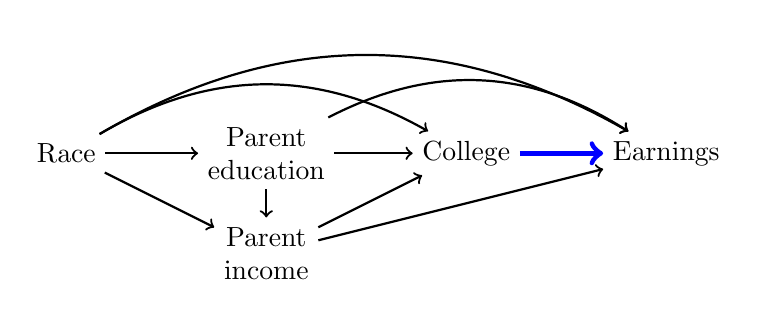
\begin{tikzpicture}[x = 1in, y = .5in]
\node (a) at (0,0) {College};
\node (y) at (1,0) {Earnings};
\node[black] (x1) at (-2,0) {Race};
\node[align = center] (x2) at (-1,0) {Parent\\education};
\node[align = center, black] (x3) at (-1,-1) {Parent\\income};
\draw[->, line width = 2pt, black, blue] (a) -- (y);
\draw[->, thick, black] (x1) to[bend left] (a);
\draw[->, thick, black] (x1) to[bend left] (y);
\draw[->, thick, black] (x1) -- (x2);
\draw[->, thick, black] (x1) -- (x3);
\draw[->, thick, black] (x2) -- (x3);
\draw[->, thick, black] (x3) -- (a);
\draw[->, thick, black] (x3) -- (y);
\draw[->, thick] (x2) -- (a);
\draw[->, thick] (x2) to[bend left] (y);
\end{tikzpicture}
\end{center}
\item Block the pathways that are not of interest
\begin{itemize}
\item e.g. estimate within subgroups of\\\{race, parent education, parent income\}
\item model-based
\begin{itemize}
\item regress earnings on everything
\item change the value of \texttt{College}
\item predict the counterfactuals
\end{itemize}
\end{itemize}
\end{enumerate}

\end{frame}

\begin{frame}{Causal inference is hard. What do we gain?}

\begin{tikzpicture}[x = \textwidth, y = .8\textheight]
\node at (0,0) {};
\node at (1,1) {};
% Individual outcomes
\node[anchor = north west, font = \bf] at (.05,1) {The data};
\foreach \i in {.5,.7,.8} {
	\draw[fill = blue, opacity = .3, color = blue] (.05,\i) rectangle (.25,\i + .1) {};
}
\foreach \i in {.3,.4,.6} {
	\draw[fill = seagreen, opacity = .3, color = seagreen] (.25,\i) rectangle (.45,\i + .1) {};
}
\node[font = \footnotesize] at (.15,.85) {$Y_\text{Nick}^\text{College}$};
\node[font = \footnotesize] at (.15,.75) {$Y_\text{William}^\text{College}$};
\node[font = \footnotesize] at (.35,.65) {$Y_\text{Rich}^\text{Non-college}$};
\node[font = \footnotesize] at (.15,.55) {$Y_\text{Diego}^\text{College}$};
\node[font = \footnotesize] at (.35,.45) {$Y_\text{Javier}^\text{Non-college}$};
\node[font = \footnotesize] at (.35,.35) {$Y_\text{Jes\'us}^\text{Non-college}$};
\node[anchor = north, align = center, font = \footnotesize, blue] at (.15, .3) {Outcome\\under\\treatment};
\node[anchor = north, align = center, font = \footnotesize, seagreen] at (.35, .3) {Outcome\\under\\control};
\node[anchor = south, rotate = 90, align = center] at (.05, .6) {Each Row is a Person};
% The claim
\node[anchor = north west, font = \bf] at (.55,1) {The claim};
\foreach \i in {.3,.4,.5,.6,.7,.8} {
	\draw[fill = blue, opacity = .3, color = blue] (.55,\i) rectangle (.75,\i + .1) {};
	\draw[fill = seagreen, opacity = .3, color = seagreen] (.75,\i) rectangle (.95,\i + .1) {};
	\draw[<->, thick] (.73,\i + .05) -- (.77,\i + .05);
}
\node[font = \footnotesize] at (.65,.85) {$Y_\text{Nick}^\text{College}$};
\node[font = \footnotesize] at (.85,.85) {$Y_\text{Nick}^\text{Non-college}$};
\node[font = \footnotesize] at (.65,.75) {$Y_\text{William}^\text{College}$};
\node[font = \footnotesize] at (.85,.75) {$Y_\text{William}^\text{Non-college}$};
\node[font = \footnotesize] at (.65,.65) {$Y_\text{Rich}^\text{College}$};
\node[font = \footnotesize] at (.85,.65) {$Y_\text{Rich}^\text{Non-college}$};
\node[font = \footnotesize] at (.65,.55) {$Y_\text{Diego}^\text{College}$};
\node[font = \footnotesize] at (.85,.55) {$Y_\text{Diego}^\text{Non-college}$};
\node[font = \footnotesize] at (.65,.45) {$Y_\text{Javier}^\text{College}$};
\node[font = \footnotesize] at (.85,.45) {$Y_\text{Javier}^\text{Non-college}$};
\node[font = \footnotesize] at (.65,.35) {$Y_\text{Jes\'us}^\text{College}$};
\node[font = \footnotesize] at (.85,.35) {$Y_\text{Jes\'us}^\text{Non-college}$};
\node[anchor = north, align = center, font = \footnotesize, blue] at (.65, .3) {Outcome\\under\\treatment};
\node[anchor = north, align = center, font = \footnotesize, seagreen] at (.85, .3) {Outcome\\under\\control};
\node[font = \footnotesize] at (.35,.85) {?};
\node[font = \footnotesize] at (.35,.75) {?};
\node[font = \footnotesize] at (.15,.65) {?};
\node[font = \footnotesize] at (.35,.55) {?};
\node[font = \footnotesize] at (.15,.45) {?};
\node[font = \footnotesize] at (.15,.35) {?};
\draw (.05,.6) rectangle (.45,.9);
\draw (.05,.3) rectangle (.45,.6);
\draw[->, thick] (.3, .68) to[out = 90, in = 215] (.33,.73);
\draw[->, thick] (.3, .68) to[out = 90, in = 215] (.33,.83);
\draw[->, thick] (.1, .83) to[out = 215, in = 150] (.13,.65);
\draw[->, thick] (.1, .73) to[out = 215, in = 150] (.13,.65);
\draw[->, thick] (.116, .53) to[out = 270, in = 150] (.14,.47);
\draw[->, thick] (.116, .53) to[out = 270, in = 150] (.14,.37);
\draw[->, thick] (.3, .47) to[out = 115, in = 210] (.33,.53);
\draw[->, thick] (.28, .37) to[out = 145, in = 210] (.33,.53);
\end{tikzpicture}
\end{frame}

\end{document}


\begin{frame}{Translate causal statements to potential outcomes}

\begin{tikzpicture}[x = \textwidth, y = .9\textheight]
\node at (0,0) {};
\node at (1,1) {};
\node<8->[anchor = north] at (.5,.9) {\bblue{Is it possible to know if each statement is true?}};
\only<2->{
\node[anchor = north west, align = left] at (0,.8) {1)};
\node[anchor = north west, align = left] at (0.05,.8) {
Sarah would have been hired\\
if she had submitted her\\
application on time
};
}
\only<3->{
\node[anchor = north east, align = right] at (1,.8) {$\begin{aligned}&Y_\text{Sarah}^\text{On time} &= 1\\&Y^\text{Late}_\text{Sarah} &= 0\end{aligned}$};
}
\only<4->{
\node[anchor = north west, align = left] at (0,.6) {2)};
\node[anchor = north west, align = left] at (0.05,.6) {
David would have been\\hired even if he hadn't\\had a college degree
};
\node[anchor = north west, align = left] at (0,.4) {3)};
\node[anchor = north west, align = left] at (0.05,.4) {
The hiring manager discriminatorily\\chose Emily over Lakisha\\because of their names
};
\node[anchor = north west, align = left] at (0,.2) {4)};
\node[anchor = north west, align = left] at (0.05,.2) {
Juan never even applied because\\
he has a newborn infant
};
}
\node<5->[anchor = north east, align = right] at (1,.6) {$\begin{aligned} &Y_\text{David}^\text{College} &= 1\\&Y_\text{David}^\text{Non-college} &= 1\end{aligned}$};
\node<6->[anchor = north east, align = right] at (1,.4) {$\begin{aligned}&Y_\text{Lakisha}^\text{Named Emily} &= 1\\&Y_\text{Lakisha}^\text{Named Lakisha} &= 0\end{aligned}$};
\node<7->[anchor = north east, align = right] at (1,.2) {$\begin{aligned}&Y_\text{Juan}^\text{Infant} &= 0\\&Y_\text{Juan}^\text{No infant} &= 1\end{aligned}$};
\end{tikzpicture}

\end{frame}

